
\section {Manutenção do PROSAC e Implementação de Aplicações Clientes}
%\subsection{Introdução}

\begin{frame}
\frametitle {\textit{Firmware} de controle PROSAC}
\framesubtitle{Introdução}

\begin{itemize}
  \item Firmware desenvolvido no Grupo de Controle.
  \item Propósito é receber requisições da sala de controle e acionar a
  respectiva placa do bastidor.
  \item Suporta diversas placas que são usadas atualmente no UVX:
  \begin{itemize}
    \item LOCON de 12 e 16 bits.
    \item STATFNT.
    \item DIGINT.
    \item \ldots
   \end{itemize}
   \item Atualmente, executado sobre o \textit{single-board computer Advantech
   PCM-4153F}:
   \begin{itemize} 
   		\item Problema: alto custo das SBCs.
   \end{itemize} 
\end{itemize}

\end{frame}

%\subsection{Manutenção do PROSAC}

\begin{frame}
\frametitle {Manutenção do PROSAC}

\begin{itemize}
  \item Migração para a \textit{BeagleBone}: solução mais barata e forte
  comunidade.
  \item Artigo na PCaPAC 2016: \textcolor{red}{\textit{UVX Control System: An
  Approach With BeagleBone Black}}.
  \item Tarefa: ajustar a política de escalonamento e a prioridade das
  \textit{threads}:
  \begin{itemize}
   \item \textit{Completely Fair Scheduler}.
   \end{itemize}
\end{itemize}

\vspace{-12pt}
\begin{table}[h]

	\centering
	\caption{\label{tab:prosac} Resultados do \textit{PROSAC} com o
	\textit{Completely Fair Scheduler}.}
	\begin{tabular}{| c | c | c | c |}
		\hline
		\textbf{Frequência (Hz)} & \textbf{Pulsos perdidos} & \textbf{Total} &
		\textbf{Razão} \\ \hline 
		150 	& 0 	& 579.812  & 0 \\ \hline
		512 	& 8 	& 5.376.056 & 0.0001\% \\ \hline
		1000 	& 18 	& 6.050.225 & 0.0003\% \\ \hline
	\end{tabular}	    
\end{table}

\end{frame}

%\subsection{Implementação de Clientes do PROSAC}

\begin{frame}
\frametitle {Implementação de Clientes do PROSAC}

\begin{itemize}
  \item Cliente em JAVA:	 
\end{itemize}

\begin{figure}
\centering
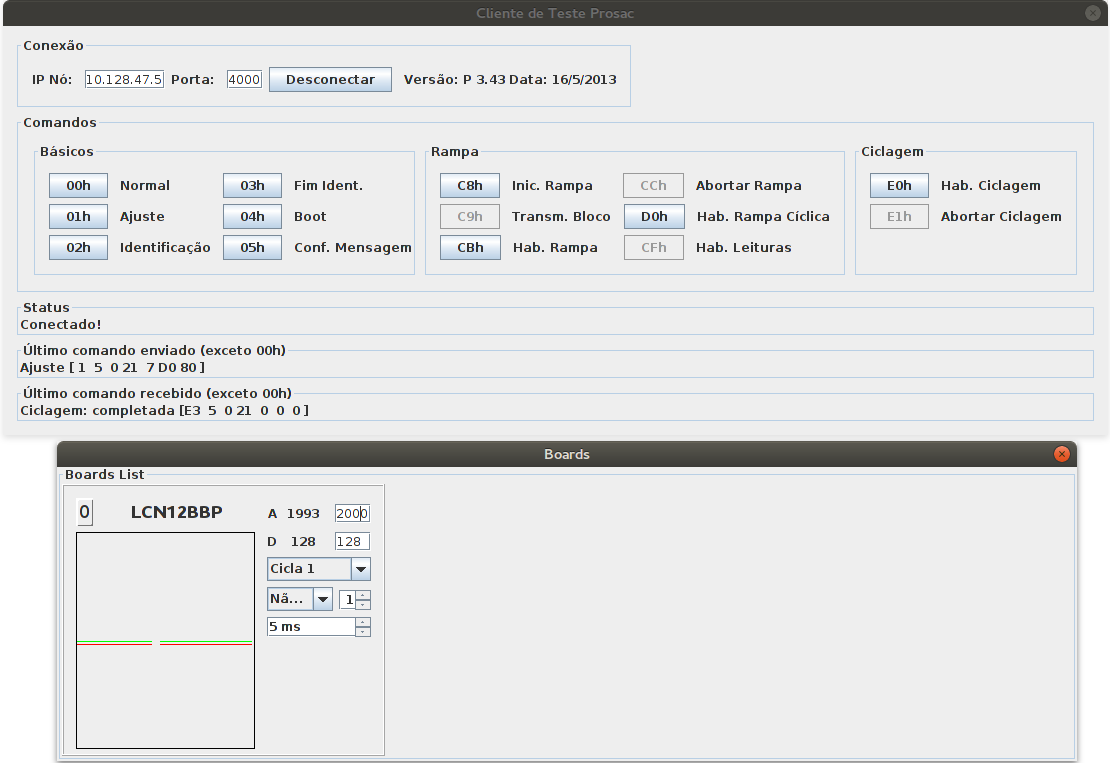
\includegraphics[width=0.7\textwidth]{image/prosac-java}
\caption {Cliente PROSAC baseado em JAVA.}
\label{fig:login}
\end{figure}
 
\end{frame}

\begin{frame}
\frametitle {Implementação de Clientes do PROSAC}

\begin{itemize}
  \item Cliente baseado no \textit{kit} \textit{STM32F7 Discovery}:	
  
  \begin{itemize} 
  \item Configuração da interface \textit{OpenOCD}.
  \item \textit{STMCubeMX} para inicialização dos pinos.
  \item \textit{FreeRTOS} e \textit{LwIP}.
  \end{itemize}
\end{itemize}

\begin{columns}
\begin{column}{0.49\textwidth}
	\begin{figure}
	\centering
	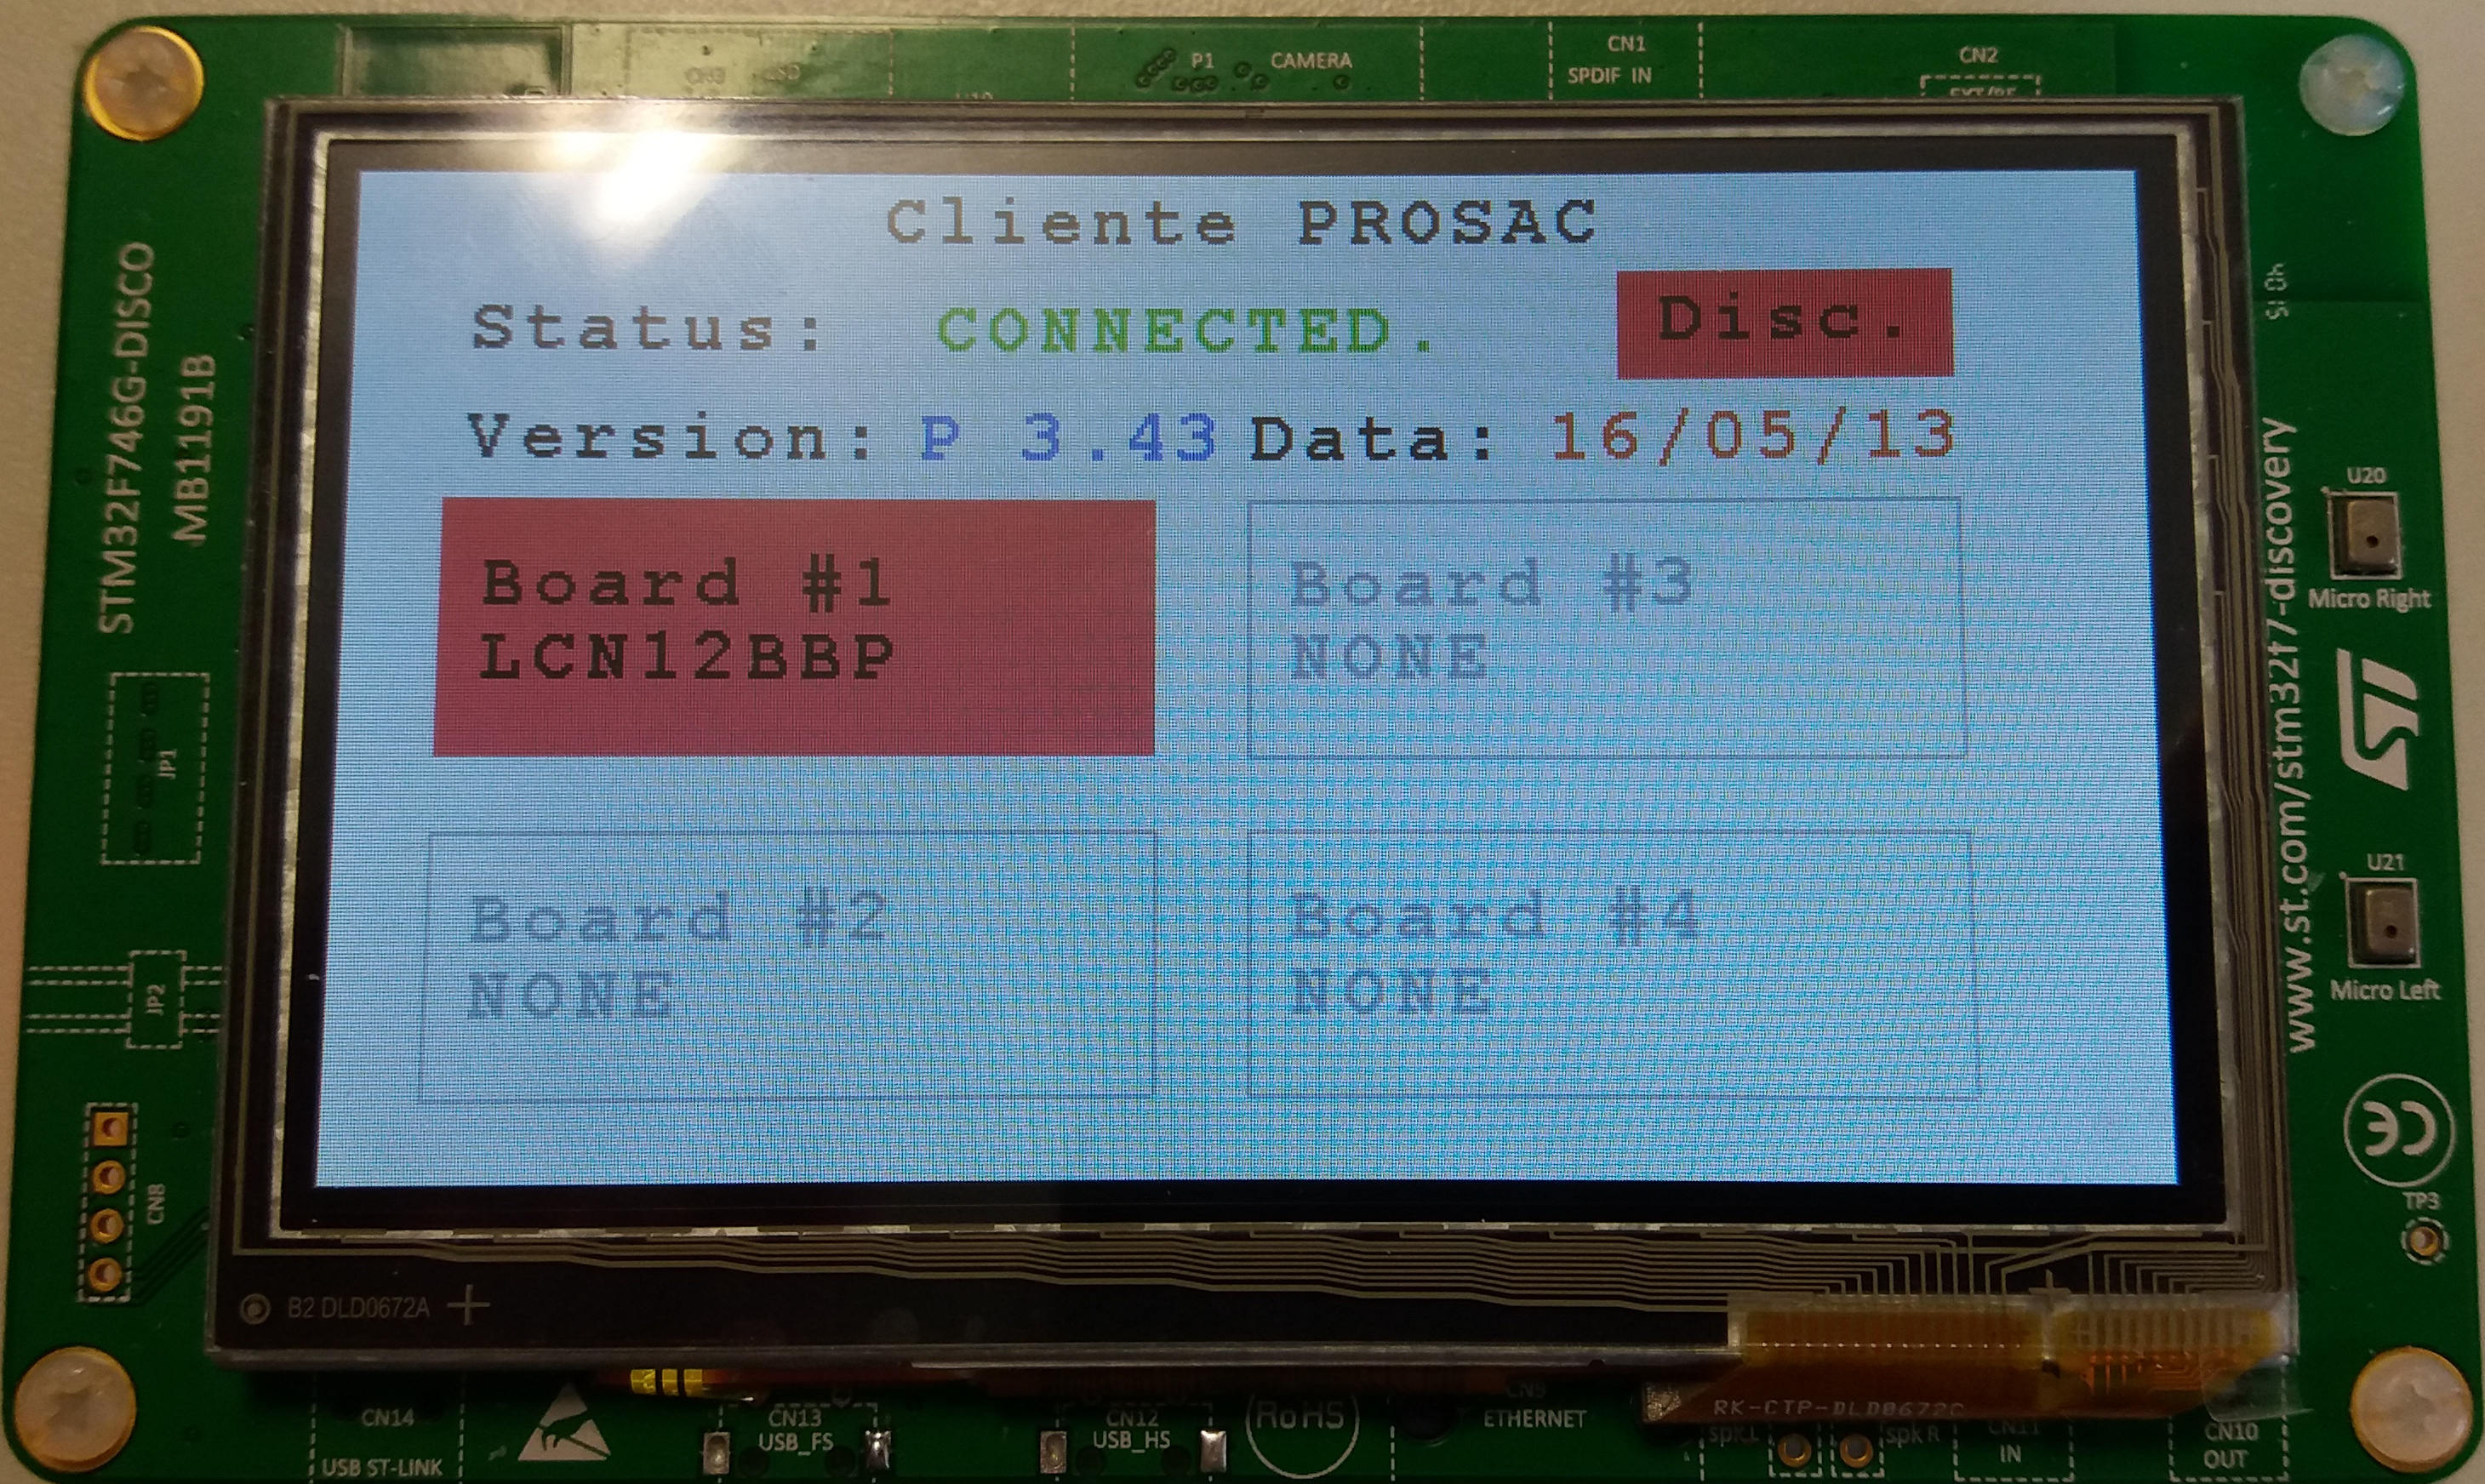
\includegraphics[width=\textwidth]{image/stm32}
	\label{fig:1}
	\caption{Tela inicial}
	\end{figure}
\end{column}
\begin{column}{0.49\textwidth}
	\begin{figure}
	\centering
	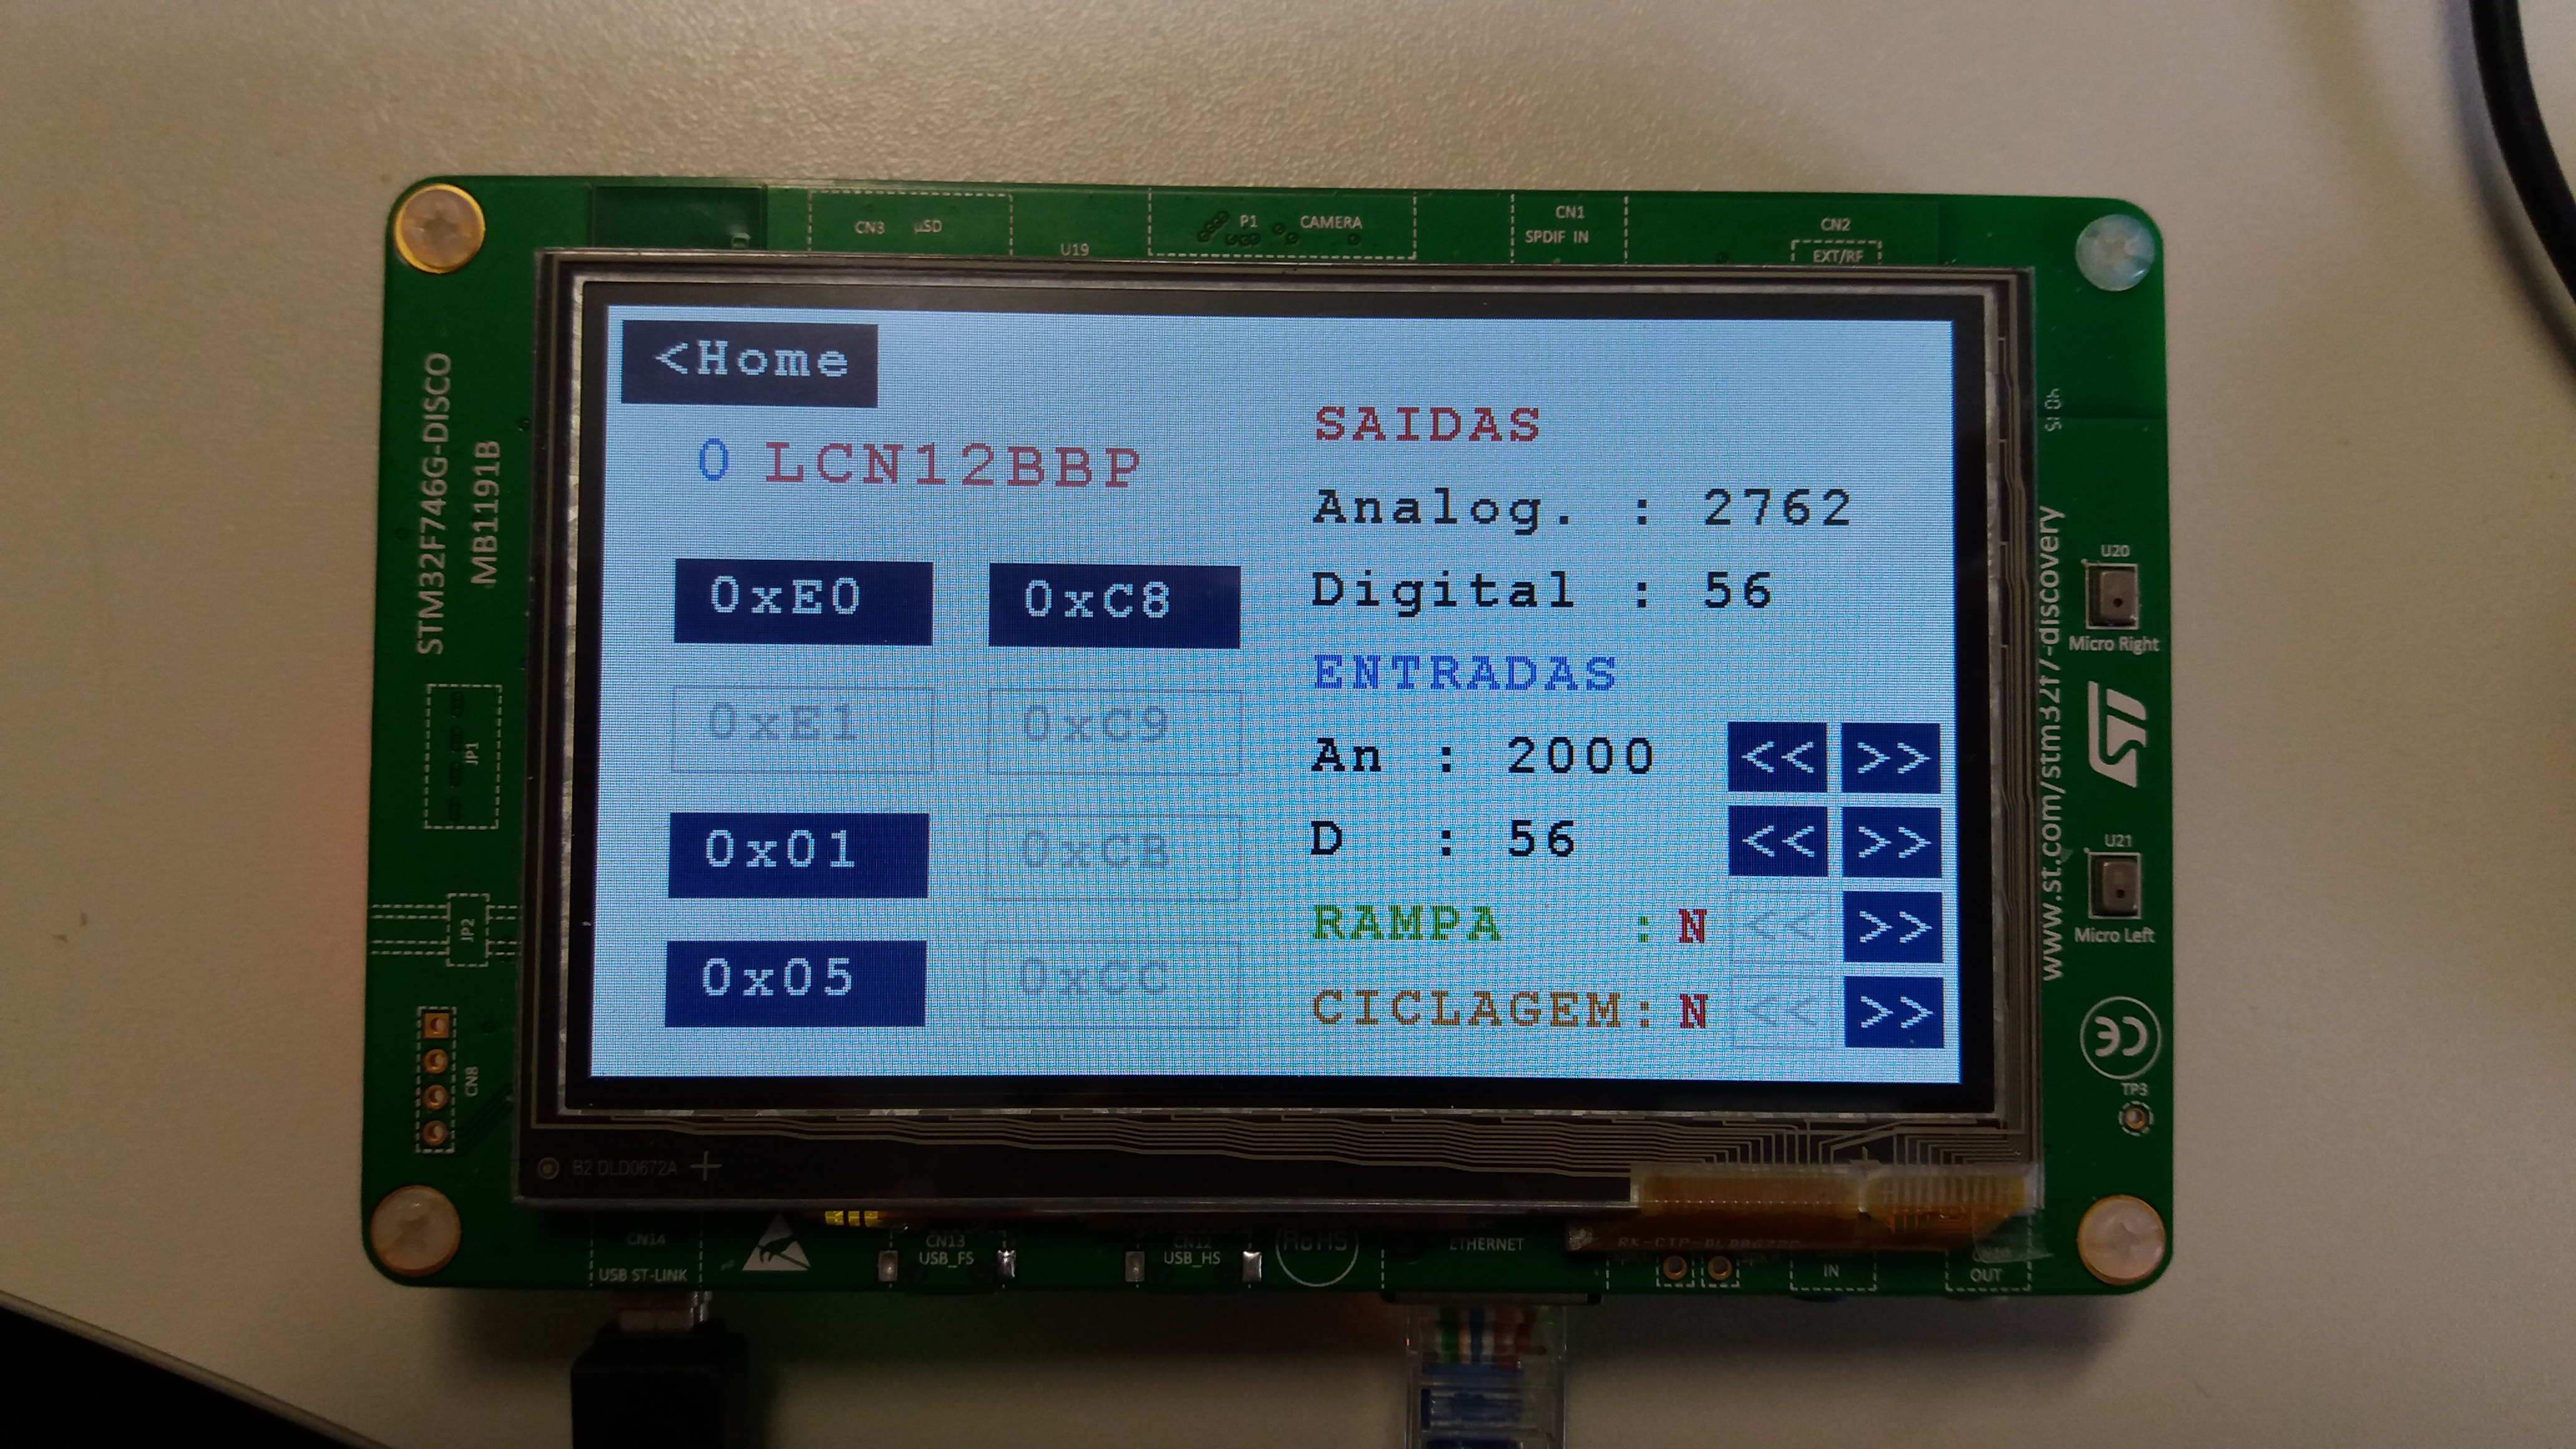
\includegraphics[width=\textwidth]{image/stm32-2}
	\label{fig:2}
	\caption {Tela de comandos}
	\end{figure}
\end{column}
\end{columns}
\end{frame}